% Options for packages loaded elsewhere
% Options for packages loaded elsewhere
\PassOptionsToPackage{unicode}{hyperref}
\PassOptionsToPackage{hyphens}{url}
\PassOptionsToPackage{dvipsnames,svgnames,x11names}{xcolor}
%
\documentclass[
  letterpaper,
  DIV=11,
  numbers=noendperiod]{scrartcl}
\usepackage{xcolor}
\usepackage{amsmath,amssymb}
\setcounter{secnumdepth}{-\maxdimen} % remove section numbering
\usepackage{iftex}
\ifPDFTeX
  \usepackage[T1]{fontenc}
  \usepackage[utf8]{inputenc}
  \usepackage{textcomp} % provide euro and other symbols
\else % if luatex or xetex
  \usepackage{unicode-math} % this also loads fontspec
  \defaultfontfeatures{Scale=MatchLowercase}
  \defaultfontfeatures[\rmfamily]{Ligatures=TeX,Scale=1}
\fi
\usepackage{lmodern}
\ifPDFTeX\else
  % xetex/luatex font selection
\fi
% Use upquote if available, for straight quotes in verbatim environments
\IfFileExists{upquote.sty}{\usepackage{upquote}}{}
\IfFileExists{microtype.sty}{% use microtype if available
  \usepackage[]{microtype}
  \UseMicrotypeSet[protrusion]{basicmath} % disable protrusion for tt fonts
}{}
\makeatletter
\@ifundefined{KOMAClassName}{% if non-KOMA class
  \IfFileExists{parskip.sty}{%
    \usepackage{parskip}
  }{% else
    \setlength{\parindent}{0pt}
    \setlength{\parskip}{6pt plus 2pt minus 1pt}}
}{% if KOMA class
  \KOMAoptions{parskip=half}}
\makeatother
% Make \paragraph and \subparagraph free-standing
\makeatletter
\ifx\paragraph\undefined\else
  \let\oldparagraph\paragraph
  \renewcommand{\paragraph}{
    \@ifstar
      \xxxParagraphStar
      \xxxParagraphNoStar
  }
  \newcommand{\xxxParagraphStar}[1]{\oldparagraph*{#1}\mbox{}}
  \newcommand{\xxxParagraphNoStar}[1]{\oldparagraph{#1}\mbox{}}
\fi
\ifx\subparagraph\undefined\else
  \let\oldsubparagraph\subparagraph
  \renewcommand{\subparagraph}{
    \@ifstar
      \xxxSubParagraphStar
      \xxxSubParagraphNoStar
  }
  \newcommand{\xxxSubParagraphStar}[1]{\oldsubparagraph*{#1}\mbox{}}
  \newcommand{\xxxSubParagraphNoStar}[1]{\oldsubparagraph{#1}\mbox{}}
\fi
\makeatother


\usepackage{longtable,booktabs,array}
\usepackage{calc} % for calculating minipage widths
% Correct order of tables after \paragraph or \subparagraph
\usepackage{etoolbox}
\makeatletter
\patchcmd\longtable{\par}{\if@noskipsec\mbox{}\fi\par}{}{}
\makeatother
% Allow footnotes in longtable head/foot
\IfFileExists{footnotehyper.sty}{\usepackage{footnotehyper}}{\usepackage{footnote}}
\makesavenoteenv{longtable}
\usepackage{graphicx}
\makeatletter
\newsavebox\pandoc@box
\newcommand*\pandocbounded[1]{% scales image to fit in text height/width
  \sbox\pandoc@box{#1}%
  \Gscale@div\@tempa{\textheight}{\dimexpr\ht\pandoc@box+\dp\pandoc@box\relax}%
  \Gscale@div\@tempb{\linewidth}{\wd\pandoc@box}%
  \ifdim\@tempb\p@<\@tempa\p@\let\@tempa\@tempb\fi% select the smaller of both
  \ifdim\@tempa\p@<\p@\scalebox{\@tempa}{\usebox\pandoc@box}%
  \else\usebox{\pandoc@box}%
  \fi%
}
% Set default figure placement to htbp
\def\fps@figure{htbp}
\makeatother


% definitions for citeproc citations
\NewDocumentCommand\citeproctext{}{}
\NewDocumentCommand\citeproc{mm}{%
  \begingroup\def\citeproctext{#2}\cite{#1}\endgroup}
\makeatletter
 % allow citations to break across lines
 \let\@cite@ofmt\@firstofone
 % avoid brackets around text for \cite:
 \def\@biblabel#1{}
 \def\@cite#1#2{{#1\if@tempswa , #2\fi}}
\makeatother
\newlength{\cslhangindent}
\setlength{\cslhangindent}{1.5em}
\newlength{\csllabelwidth}
\setlength{\csllabelwidth}{3em}
\newenvironment{CSLReferences}[2] % #1 hanging-indent, #2 entry-spacing
 {\begin{list}{}{%
  \setlength{\itemindent}{0pt}
  \setlength{\leftmargin}{0pt}
  \setlength{\parsep}{0pt}
  % turn on hanging indent if param 1 is 1
  \ifodd #1
   \setlength{\leftmargin}{\cslhangindent}
   \setlength{\itemindent}{-1\cslhangindent}
  \fi
  % set entry spacing
  \setlength{\itemsep}{#2\baselineskip}}}
 {\end{list}}
\usepackage{calc}
\newcommand{\CSLBlock}[1]{\hfill\break\parbox[t]{\linewidth}{\strut\ignorespaces#1\strut}}
\newcommand{\CSLLeftMargin}[1]{\parbox[t]{\csllabelwidth}{\strut#1\strut}}
\newcommand{\CSLRightInline}[1]{\parbox[t]{\linewidth - \csllabelwidth}{\strut#1\strut}}
\newcommand{\CSLIndent}[1]{\hspace{\cslhangindent}#1}



\setlength{\emergencystretch}{3em} % prevent overfull lines

\providecommand{\tightlist}{%
  \setlength{\itemsep}{0pt}\setlength{\parskip}{0pt}}



 


\KOMAoption{captions}{tableheading}
\makeatletter
\@ifpackageloaded{caption}{}{\usepackage{caption}}
\AtBeginDocument{%
\ifdefined\contentsname
  \renewcommand*\contentsname{Table of contents}
\else
  \newcommand\contentsname{Table of contents}
\fi
\ifdefined\listfigurename
  \renewcommand*\listfigurename{List of Figures}
\else
  \newcommand\listfigurename{List of Figures}
\fi
\ifdefined\listtablename
  \renewcommand*\listtablename{List of Tables}
\else
  \newcommand\listtablename{List of Tables}
\fi
\ifdefined\figurename
  \renewcommand*\figurename{Figure}
\else
  \newcommand\figurename{Figure}
\fi
\ifdefined\tablename
  \renewcommand*\tablename{Table}
\else
  \newcommand\tablename{Table}
\fi
}
\@ifpackageloaded{float}{}{\usepackage{float}}
\floatstyle{ruled}
\@ifundefined{c@chapter}{\newfloat{codelisting}{h}{lop}}{\newfloat{codelisting}{h}{lop}[chapter]}
\floatname{codelisting}{Listing}
\newcommand*\listoflistings{\listof{codelisting}{List of Listings}}
\makeatother
\makeatletter
\makeatother
\makeatletter
\@ifpackageloaded{caption}{}{\usepackage{caption}}
\@ifpackageloaded{subcaption}{}{\usepackage{subcaption}}
\makeatother
\usepackage{bookmark}
\IfFileExists{xurl.sty}{\usepackage{xurl}}{} % add URL line breaks if available
\urlstyle{same}
\hypersetup{
  pdftitle={Predicting Movie Revenue From Movie Budget},
  pdfauthor={Audrey Vo, Roxanna Ng, Nikita Prabhu, Philip Chen},
  colorlinks=true,
  linkcolor={blue},
  filecolor={Maroon},
  citecolor={Blue},
  urlcolor={Blue},
  pdfcreator={LaTeX via pandoc}}


\title{Predicting Movie Revenue From Movie Budget}
\author{Audrey Vo, Roxanna Ng, Nikita Prabhu, Philip Chen}
\date{}
\begin{document}
\maketitle


\section{Summary}\label{summary}

This study investigates how movie budget predicts domestic box office
revenue using the Bechdel Test movie dataset from FiveThirtyEight.
Exploratory anaylsis revealed right-skewed distributions for both budget
and revenue, which were log-transformed to stabilize variance. A linear
regression model and a K-nearest neighbours (KNN) regression model were
fitted to predict log-transformed domestic revenue from log-transformed
movie budget. Both models showed moderate predictive performance, with a
root mean squared prediction error (RMSPE) of roughly 1.27 and 1.29 log
units, respectively. The results suggest that while higher budgets are
generally associated with higher revenue, budget alone cannot fully
explain the variability in box office performance. These findings
highlight the complexity of film revenue prediction and the importance
of incorporating additional factors beyond production budget.

\section{Introduction}\label{introduction}

The financial performance of a film is often assumed to be strongly
related to its production budget. Higher budgets allow studios to invest
in elements such as well-known actors, special effects, marketing
campaigns, and larger production teams, which are often assumed to
influence audience appeal and box office revenue (Basuroy, Chatterjee,
and Ravid 2003). However, the extent to which movie budgets actually
predict revenue remains uncertain, as many lower-budget films have seen
significant success in the box office while some high-budget productions
fail to recover the costs associated with making the movie (De Vany and
Walls 1999).

Understanding the relationship between production budget and revenue can
provide insight into whether increased financial investments reliably
leads to higher financial returns.

\subsection{Research Question}\label{research-question}

How does movie budget predict movie revenue?

\subsection{The Data Set}\label{the-data-set}

In this analysis, we use FiveThirtyEight's Bechdel Test dataset, which
contains descriptive information, production budgets and domestic box
office revenue of 1,615 films released between 1990 and 2013 to answer
our research question (FiveThirtyEight 2014).

Here, we take a look at the first couple rows of the raw data.

\begin{longtable}[]{@{}
  >{\raggedleft\arraybackslash}p{(\linewidth - 28\tabcolsep) * \real{0.0294}}
  >{\raggedright\arraybackslash}p{(\linewidth - 28\tabcolsep) * \real{0.0588}}
  >{\raggedright\arraybackslash}p{(\linewidth - 28\tabcolsep) * \real{0.1000}}
  >{\raggedright\arraybackslash}p{(\linewidth - 28\tabcolsep) * \real{0.0941}}
  >{\raggedright\arraybackslash}p{(\linewidth - 28\tabcolsep) * \real{0.0647}}
  >{\raggedright\arraybackslash}p{(\linewidth - 28\tabcolsep) * \real{0.0412}}
  >{\raggedleft\arraybackslash}p{(\linewidth - 28\tabcolsep) * \real{0.0529}}
  >{\raggedright\arraybackslash}p{(\linewidth - 28\tabcolsep) * \real{0.0529}}
  >{\raggedright\arraybackslash}p{(\linewidth - 28\tabcolsep) * \real{0.0588}}
  >{\raggedright\arraybackslash}p{(\linewidth - 28\tabcolsep) * \real{0.0529}}
  >{\raggedleft\arraybackslash}p{(\linewidth - 28\tabcolsep) * \real{0.0765}}
  >{\raggedright\arraybackslash}p{(\linewidth - 28\tabcolsep) * \real{0.0882}}
  >{\raggedright\arraybackslash}p{(\linewidth - 28\tabcolsep) * \real{0.0882}}
  >{\raggedleft\arraybackslash}p{(\linewidth - 28\tabcolsep) * \real{0.0706}}
  >{\raggedleft\arraybackslash}p{(\linewidth - 28\tabcolsep) * \real{0.0706}}@{}}

\caption{\label{tbl-movie-data-raw}First 6 rows of the raw data}

\tabularnewline

\toprule\noalign{}
\begin{minipage}[b]{\linewidth}\raggedleft
year
\end{minipage} & \begin{minipage}[b]{\linewidth}\raggedright
imdb
\end{minipage} & \begin{minipage}[b]{\linewidth}\raggedright
title
\end{minipage} & \begin{minipage}[b]{\linewidth}\raggedright
test
\end{minipage} & \begin{minipage}[b]{\linewidth}\raggedright
clean\_test
\end{minipage} & \begin{minipage}[b]{\linewidth}\raggedright
binary
\end{minipage} & \begin{minipage}[b]{\linewidth}\raggedleft
budget
\end{minipage} & \begin{minipage}[b]{\linewidth}\raggedright
domgross
\end{minipage} & \begin{minipage}[b]{\linewidth}\raggedright
intgross
\end{minipage} & \begin{minipage}[b]{\linewidth}\raggedright
code
\end{minipage} & \begin{minipage}[b]{\linewidth}\raggedleft
budget\_2013.
\end{minipage} & \begin{minipage}[b]{\linewidth}\raggedright
domgross\_2013.
\end{minipage} & \begin{minipage}[b]{\linewidth}\raggedright
intgross\_2013.
\end{minipage} & \begin{minipage}[b]{\linewidth}\raggedleft
period.code
\end{minipage} & \begin{minipage}[b]{\linewidth}\raggedleft
decade.code
\end{minipage} \\
\midrule\noalign{}
\endhead
\bottomrule\noalign{}
\endlastfoot
2013 & tt1711425 & 21 \& Over & notalk & notalk & FAIL & 1.30e+07 &
25682380 & 42195766 & 2013FAIL & 13000000 & 25682380 & 42195766 & 1 &
1 \\
2012 & tt1343727 & Dredd 3D & ok-disagree & ok & PASS & 4.50e+07 &
13414714 & 40868994 & 2012PASS & 45658735 & 13611086 & 41467257 & 1 &
1 \\
2013 & tt2024544 & 12 Years a Slave & notalk-disagree & notalk & FAIL &
2.00e+07 & 53107035 & 158607035 & 2013FAIL & 20000000 & 53107035 &
158607035 & 1 & 1 \\
2013 & tt1272878 & 2 Guns & notalk & notalk & FAIL & 6.10e+07 & 75612460
& 132493015 & 2013FAIL & 61000000 & 75612460 & 132493015 & 1 & 1 \\
2013 & tt0453562 & 42 & men & men & FAIL & 4.00e+07 & 95020213 &
95020213 & 2013FAIL & 40000000 & 95020213 & 95020213 & 1 & 1 \\
2013 & tt1335975 & 47 Ronin & men & men & FAIL & 2.25e+08 & 38362475 &
145803842 & 2013FAIL & 225000000 & 38362475 & 145803842 & 1 & 1 \\

\end{longtable}

\subsection{Cleaning Data}\label{cleaning-data}

Since our research question only requires studying 2 variables (movie
budget - ``budget'', movie revenue - ``domgross''), we will filter the
data to only observe those 2 columns during our analysis.

\begin{longtable}[]{@{}rr@{}}

\caption{\label{tbl-movie-data-cleaned}First 6 rows of the data}

\tabularnewline

\toprule\noalign{}
budget & domgross \\
\midrule\noalign{}
\endhead
\bottomrule\noalign{}
\endlastfoot
1.30e+07 & 25682380 \\
4.50e+07 & 13414714 \\
2.00e+07 & 53107035 \\
6.10e+07 & 75612460 \\
4.00e+07 & 95020213 \\
2.25e+08 & 38362475 \\

\end{longtable}

Next, we will check our data for any null values and filter them out if
there are any.

\begin{verbatim}
# of null values (before filtering): 17
\end{verbatim}

\begin{verbatim}
# of null values (after filtering): 0
\end{verbatim}

We will also check for any budget/revenue with a value of 0, since any
movie with a \$0 budget/revenue is most likely missing data. In
checking, we found that before filtering, there was 0 movies with no
budget and 1 movie with no revenue.

After seeing there is one entry with a non-zero budget but \$0 revenue,
we will first check to see what this value looks like. Since the value
has a very high budget, we will say this entry is most likely having its
appropriate budget missing and filter it out of the data set.

\begin{longtable}[]{@{}rr@{}}

\caption{\label{tbl-movie-data-rev}Movies with a \$0 revenue}

\tabularnewline

\toprule\noalign{}
budget & domgross \\
\midrule\noalign{}
\endhead
\bottomrule\noalign{}
\endlastfoot
1.8e+07 & 0 \\

\end{longtable}

\section{EDA}\label{eda}

Here, we will look at some general summary statistics of our data:

\begin{longtable}[]{@{}lrr@{}}

\caption{\label{tbl-eda-summary}Summary statistics of the cleaned movie
dataset}

\tabularnewline

\toprule\noalign{}
X & budget & domgross \\
\midrule\noalign{}
\endhead
\bottomrule\noalign{}
\endlastfoot
Min. & 7000 & 828 \\
1st Qu. & 12000000 & 16320870 \\
Median & 30000000 & 42239614 \\
Mean & 45174408 & 69170974 \\
3rd Qu. & 60000000 & 93382814 \\
Max. & 425000000 & 760507625 \\

\end{longtable}

Here, we will look at the general shape/values in our data:

\begin{longtable}[]{@{}ll@{}}

\caption{\label{tbl-eda-str}Structure of the cleaned movie dataset}

\tabularnewline

\toprule\noalign{}
budget & domgross \\
\midrule\noalign{}
\endhead
\bottomrule\noalign{}
\endlastfoot
numeric & numeric \\

\end{longtable}

Next, we will use different plots to examine the skew/behaviour of
budget and revenue in the data.

In Figure~\ref{fig-eda-boxplots}, we can see there is a heavy right skew
in both variables, seeing as most of the movies are clustered at the
bottom with only few movies pulling the tail towards higher values.

\begin{figure}

\centering{

\pandocbounded{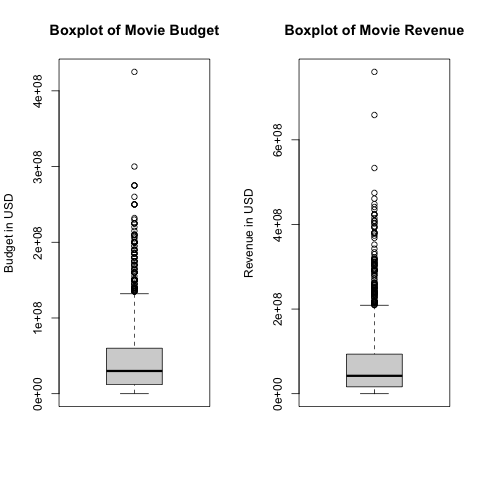
\includegraphics[keepaspectratio]{../results/figure1-eda_boxplot.png}}

}

\caption{\label{fig-eda-boxplots}Boxplots of Movie Budget and Revenue}

\end{figure}%

In Figure~\ref{fig-eda-histograms}, we can once again observe how both
variance are heavily right skewed, and like in the box plots above, we
see only some movies with higher values which indicates we have some
outliers in our data. In addition, after seeing both the box plot and
histogram, we observe that the values have a very wide range and spread.

\begin{figure}

\centering{

\pandocbounded{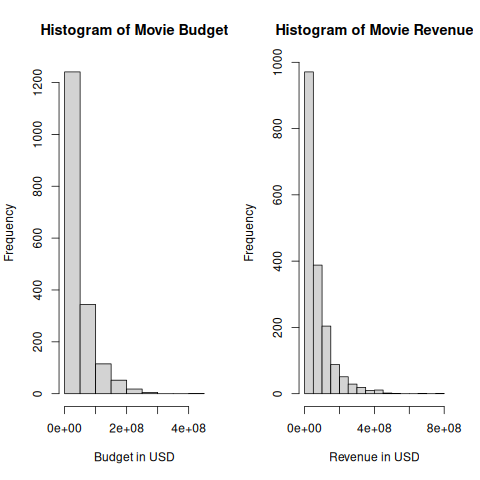
\includegraphics[keepaspectratio]{../results/figure2-eda_histogram.png}}

}

\caption{\label{fig-eda-histograms}Histograms of Movie Budget and
Revenue}

\end{figure}%

Next, we will look at the behaviour of movie budget with movie revenue
on the untransformed data to help us gather an idea of how linear the
relationship may be. From observing Figure~\ref{fig-eda-rev-vs-bud}, we
can see that the data may have a positive linear relationship. The
spread of the values are also very wide, making it difficult to conclude
how strong this linear relationship may be.

\begin{figure}

\centering{

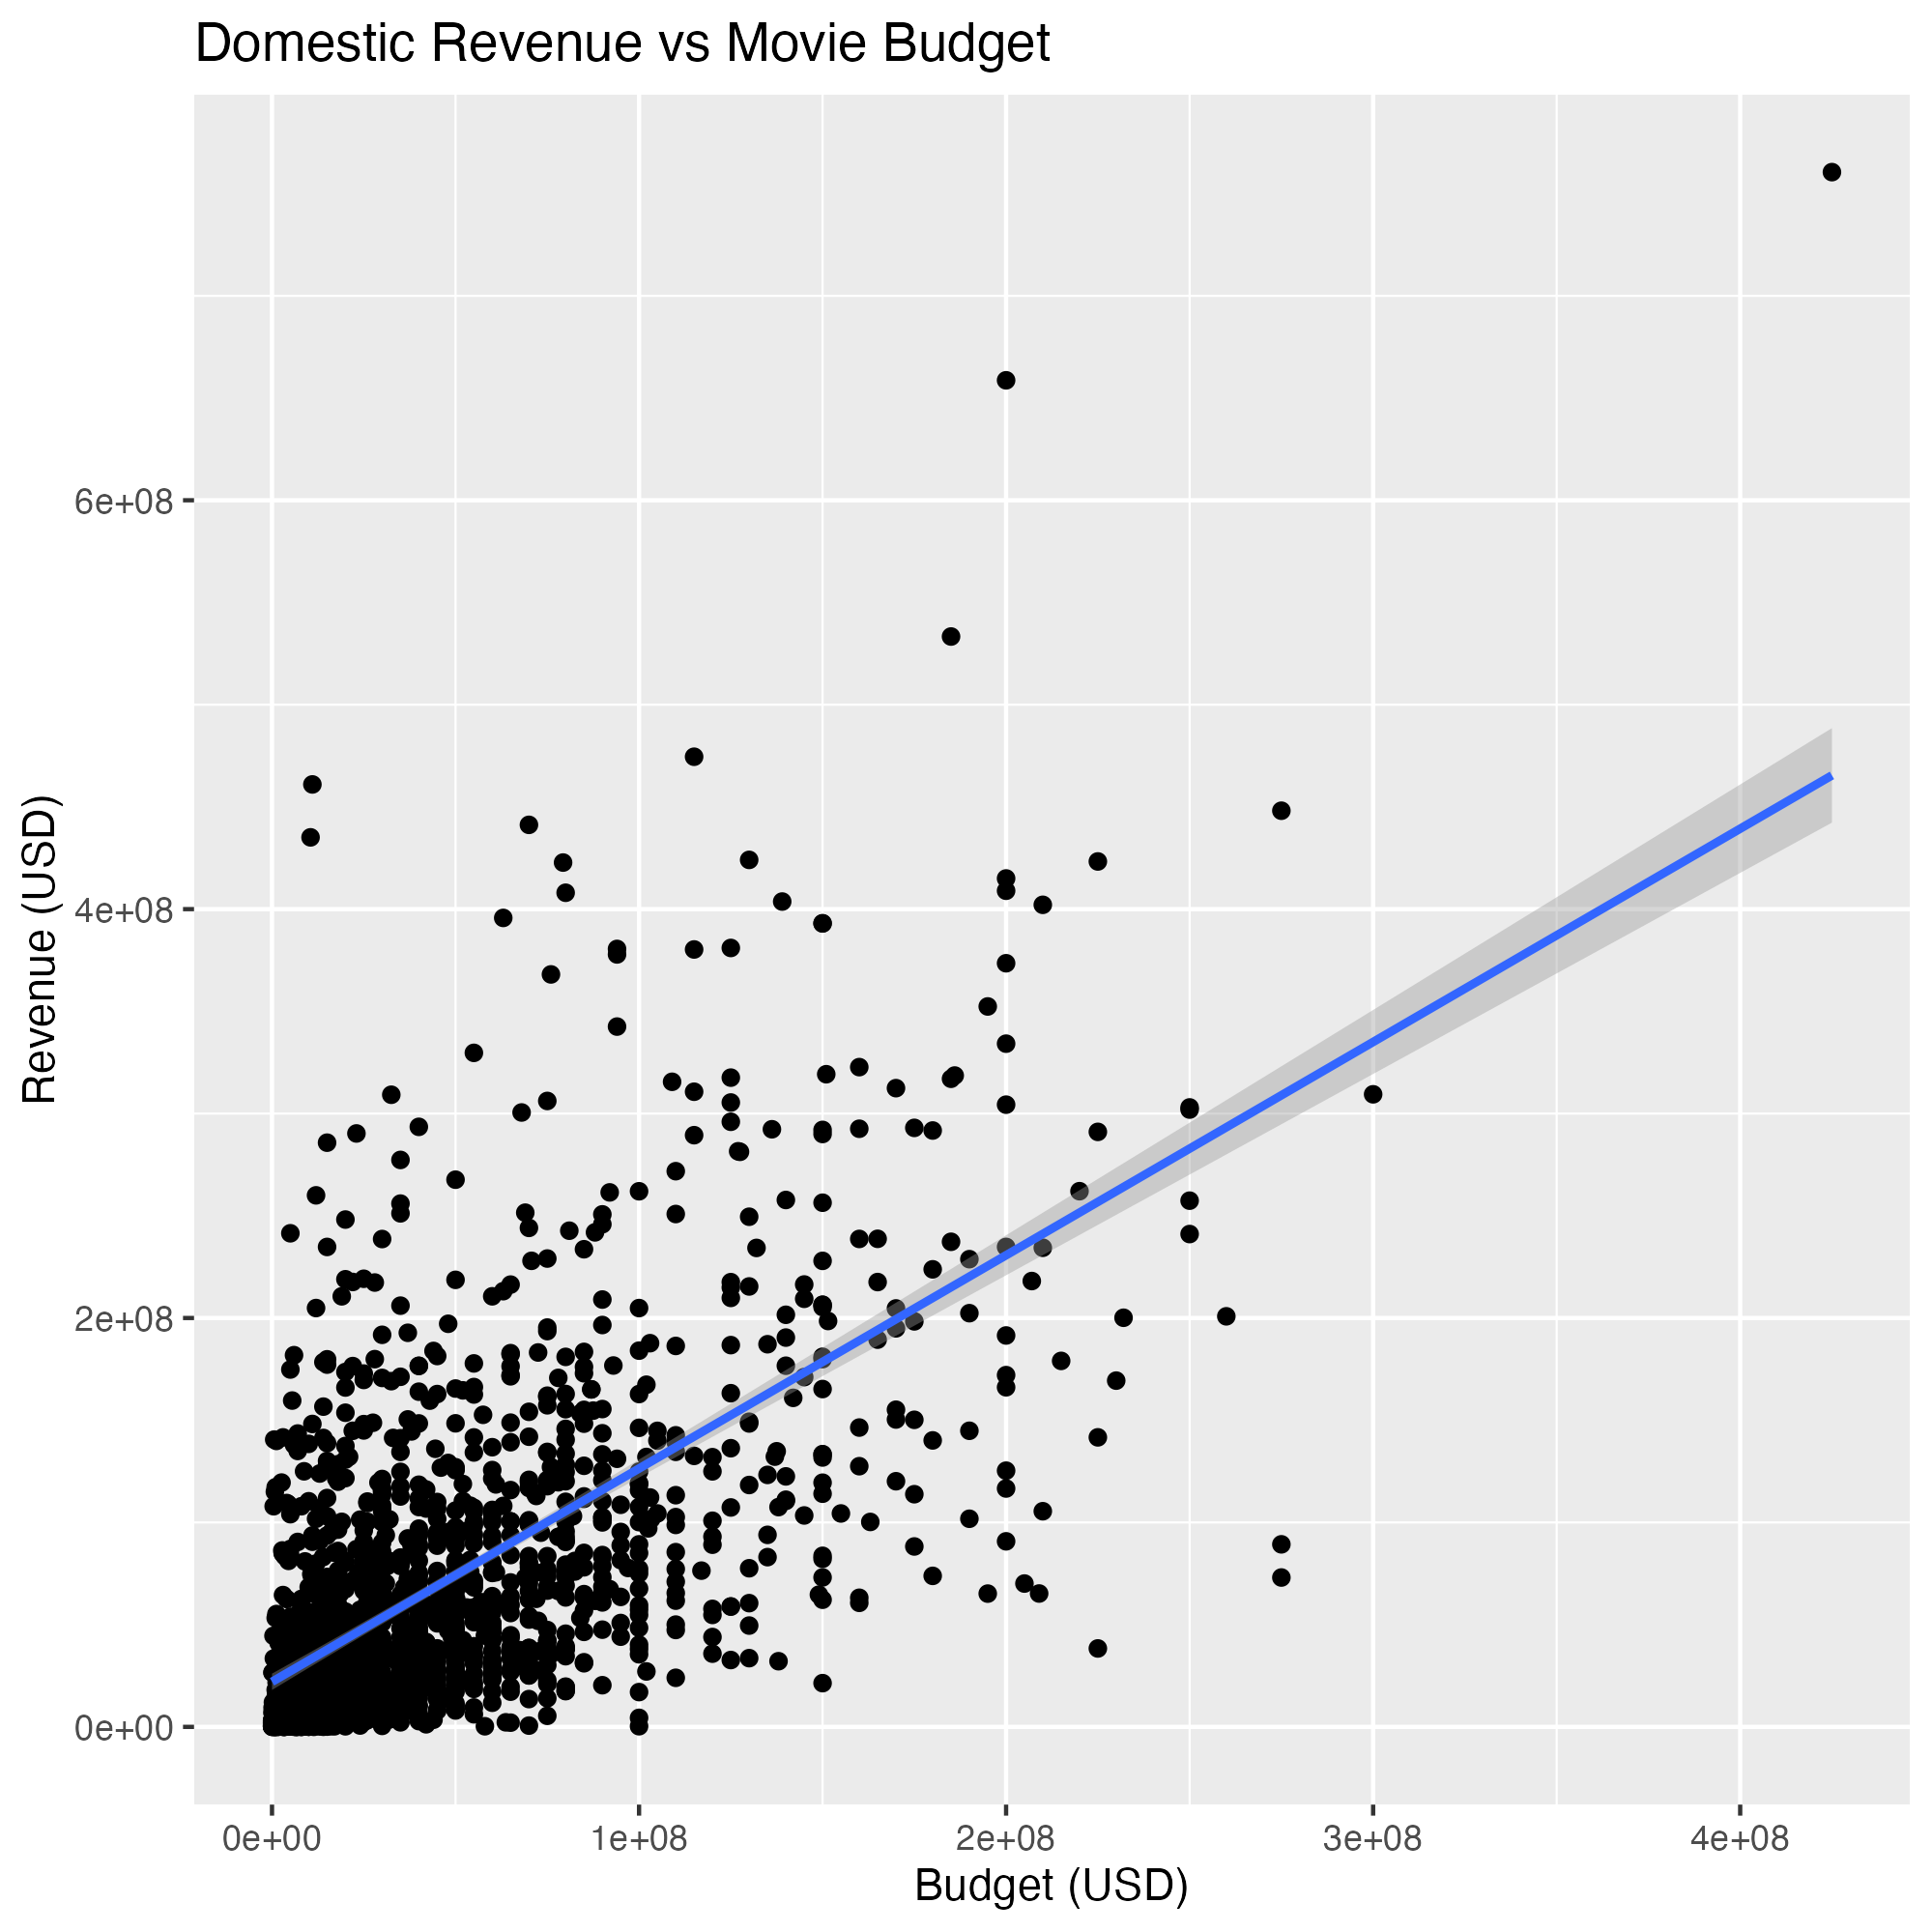
\includegraphics[width=0.65\linewidth,height=4.16667in]{../results/figure3-eda_revenue_vs_budget.png}

}

\caption{\label{fig-eda-rev-vs-bud}Scatterplot of Domestic Revenue vs
Movie Budget}

\end{figure}%

Since just observing the scatter plot makes it difficult to conclude how
linear our data is, we can observe the correlation between movie budget
and revenue. We can see that we have a correlation of around 0.627,
indicating that there may be a moderate positive relationship between
our two variables. This correlation value allows us to further our
analysis to see how well movie budget may predict movie revenue.

Previously, we observed a very large spread. To account for this, we
will apply a variance stabilizing function (log) to our variables to
help stabilize the wide range of values. We can see in
Figure~\ref{fig-eda-log-scatter} that applying this function helps make
the data less spread out and easier to observe for patterns.

\begin{figure}

\centering{

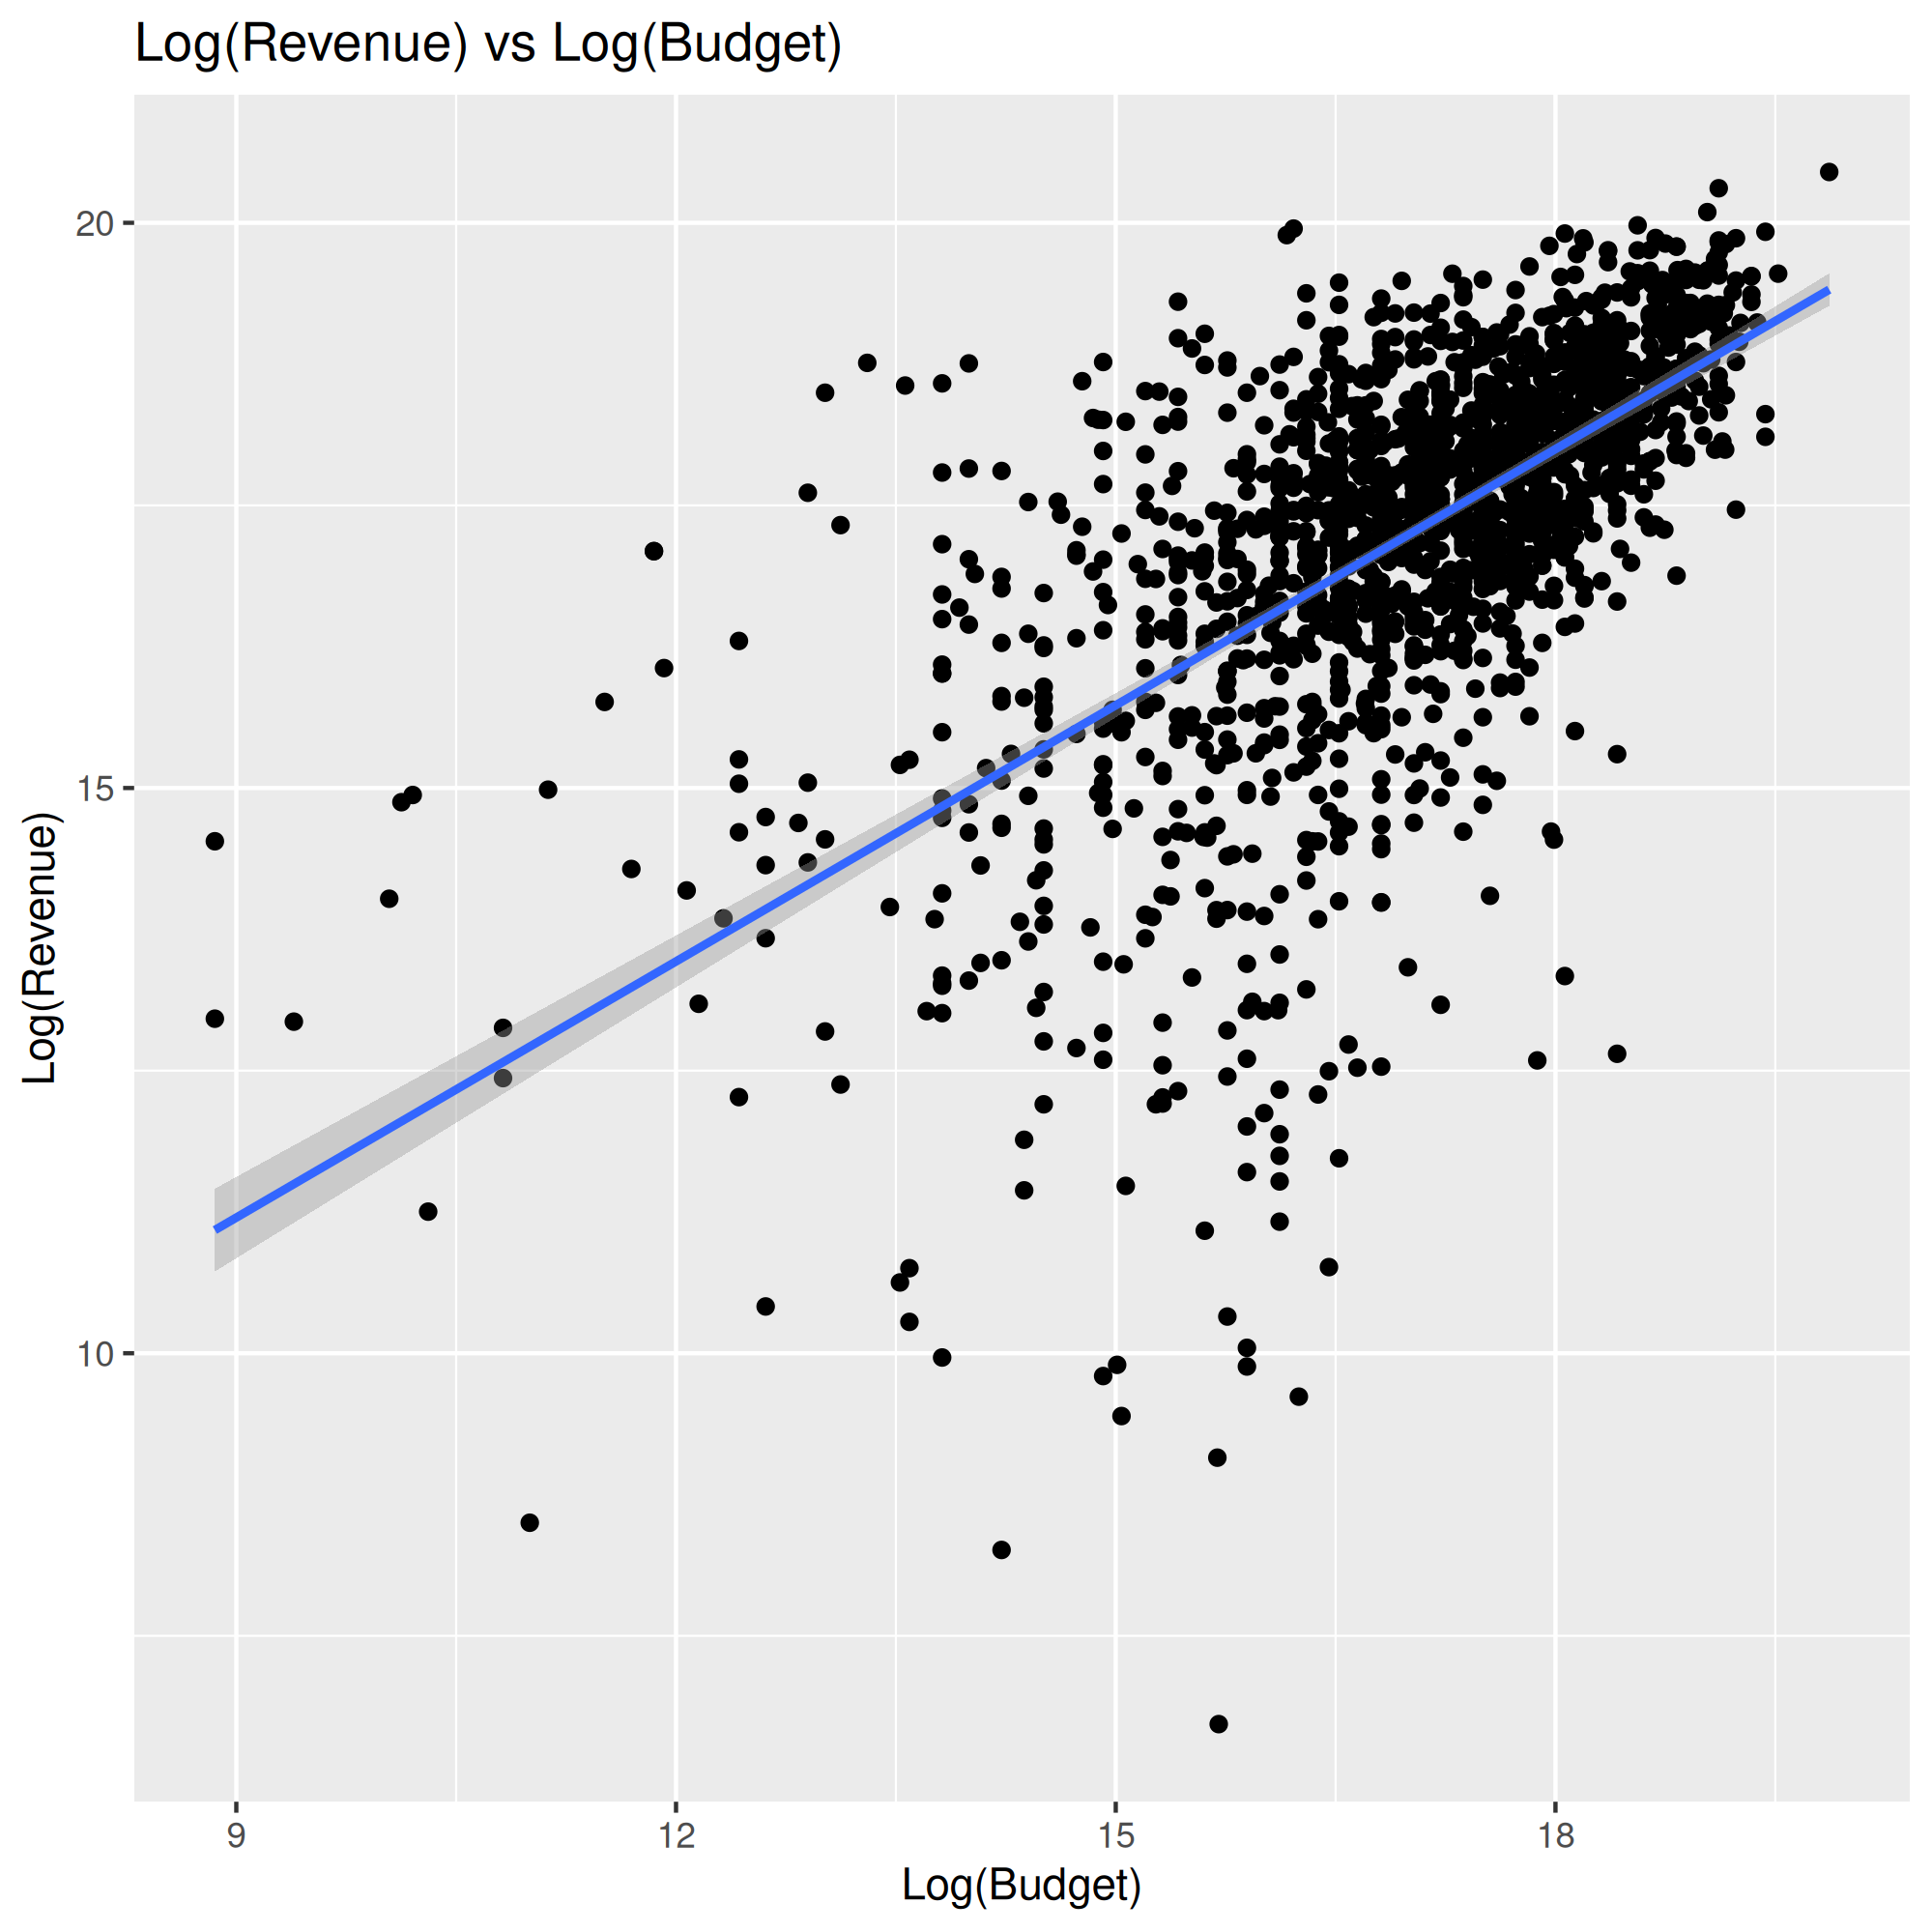
\includegraphics[width=0.65\linewidth,height=4.16667in]{../results/figure4-eda_log_revenue_vs_log_budget.png}

}

\caption{\label{fig-eda-log-scatter}Scatterplot of log(Domestic Revenue)
vs log(Movie Budget)}

\end{figure}%

Here is our data with the log-transformed budget and revenue added:

\begin{longtable}[]{@{}rrrr@{}}

\caption{\label{tbl-movie-data-log}First six rows with budget, domestic
gross, and their log-transformed values}

\tabularnewline

\toprule\noalign{}
budget & domgross & log\_budget & log\_domgross \\
\midrule\noalign{}
\endhead
\bottomrule\noalign{}
\endlastfoot
1.30e+07 & 25682380 & 16.38046 & 17.06132 \\
4.50e+07 & 13414714 & 17.62217 & 16.41186 \\
2.00e+07 & 53107035 & 16.81124 & 17.78782 \\
6.10e+07 & 75612460 & 17.92638 & 18.14113 \\
4.00e+07 & 95020213 & 17.50439 & 18.36960 \\
2.25e+08 & 38362475 & 19.23161 & 17.46259 \\

\end{longtable}

\section{Methods and Results}\label{methods-and-results}

Due to the relationship between movie budget and movie revenue being
relatively linear, we will use a linear regression for analysis. Below,
we split the data and summarize the number of observations in each
training and test split. We also look at the mean values for the
log-transformed budget and revenue columns in each training and test
split.

\begin{longtable}[]{@{}rr@{}}

\caption{\label{tbl-train-mean}Mean log-budget and log-domestic revenue
for the training set}

\tabularnewline

\toprule\noalign{}
train\_log\_budget\_mean & train\_log\_domgross\_mean \\
\midrule\noalign{}
\endhead
\bottomrule\noalign{}
\endlastfoot
16.98953 & 17.24123 \\

\end{longtable}

\begin{longtable}[]{@{}rr@{}}

\caption{\label{tbl-test-mean}Mean log-budget and log-domestic revenue
for the test set}

\tabularnewline

\toprule\noalign{}
test\_log\_budget\_mean & test\_log\_domgross\_mean \\
\midrule\noalign{}
\endhead
\bottomrule\noalign{}
\endlastfoot
16.9104 & 17.16077 \\

\end{longtable}

Below we fit a simple linear regression with the log-transformed
versions of movie budget and movie revenue to account for data skew. The
predictor (log-transformed movie budget) is statistically significant.

\begin{verbatim}

Call:
lm(formula = log_domgross ~ log_budget, data = train)

Residuals:
    Min      1Q  Median      3Q     Max 
-9.5448 -0.5775  0.1807  0.7754  4.3182 

Coefficients:
            Estimate Std. Error t value Pr(>|t|)    
(Intercept)  4.33845    0.48805   8.889   <2e-16 ***
log_budget   0.75945    0.02863  26.524   <2e-16 ***
---
Signif. codes:  0 ‘***’ 0.001 ‘**’ 0.01 ‘*’ 0.05 ‘.’ 0.1 ‘ ’ 1

Residual standard error: 1.391 on 1241 degrees of freedom
Multiple R-squared:  0.3618,    Adjusted R-squared:  0.3613 
F-statistic: 703.5 on 1 and 1241 DF,  p-value: < 2.2e-16
\end{verbatim}

Using the fitted model above, we predict on the test set.

\begin{longtable}[]{@{}rrr@{}}

\caption{\label{tbl-lm-preds}Predicted log domestic revenue with the
corresponding log-budget and actual log-domestic revenue for test set}

\tabularnewline

\toprule\noalign{}
log\_domgross\_preds & log\_budget & log\_domgross \\
\midrule\noalign{}
\endhead
\bottomrule\noalign{}
\endlastfoot
17.72169 & 17.62217 & 16.41186 \\
17.27529 & 17.03439 & 17.43463 \\
17.41376 & 17.21671 & 17.37845 \\
18.40050 & 18.51599 & 17.93840 \\
16.98240 & 16.64872 & 17.80893 \\
16.05300 & 15.42495 & 18.24139 \\

\end{longtable}

\begin{figure}

\centering{

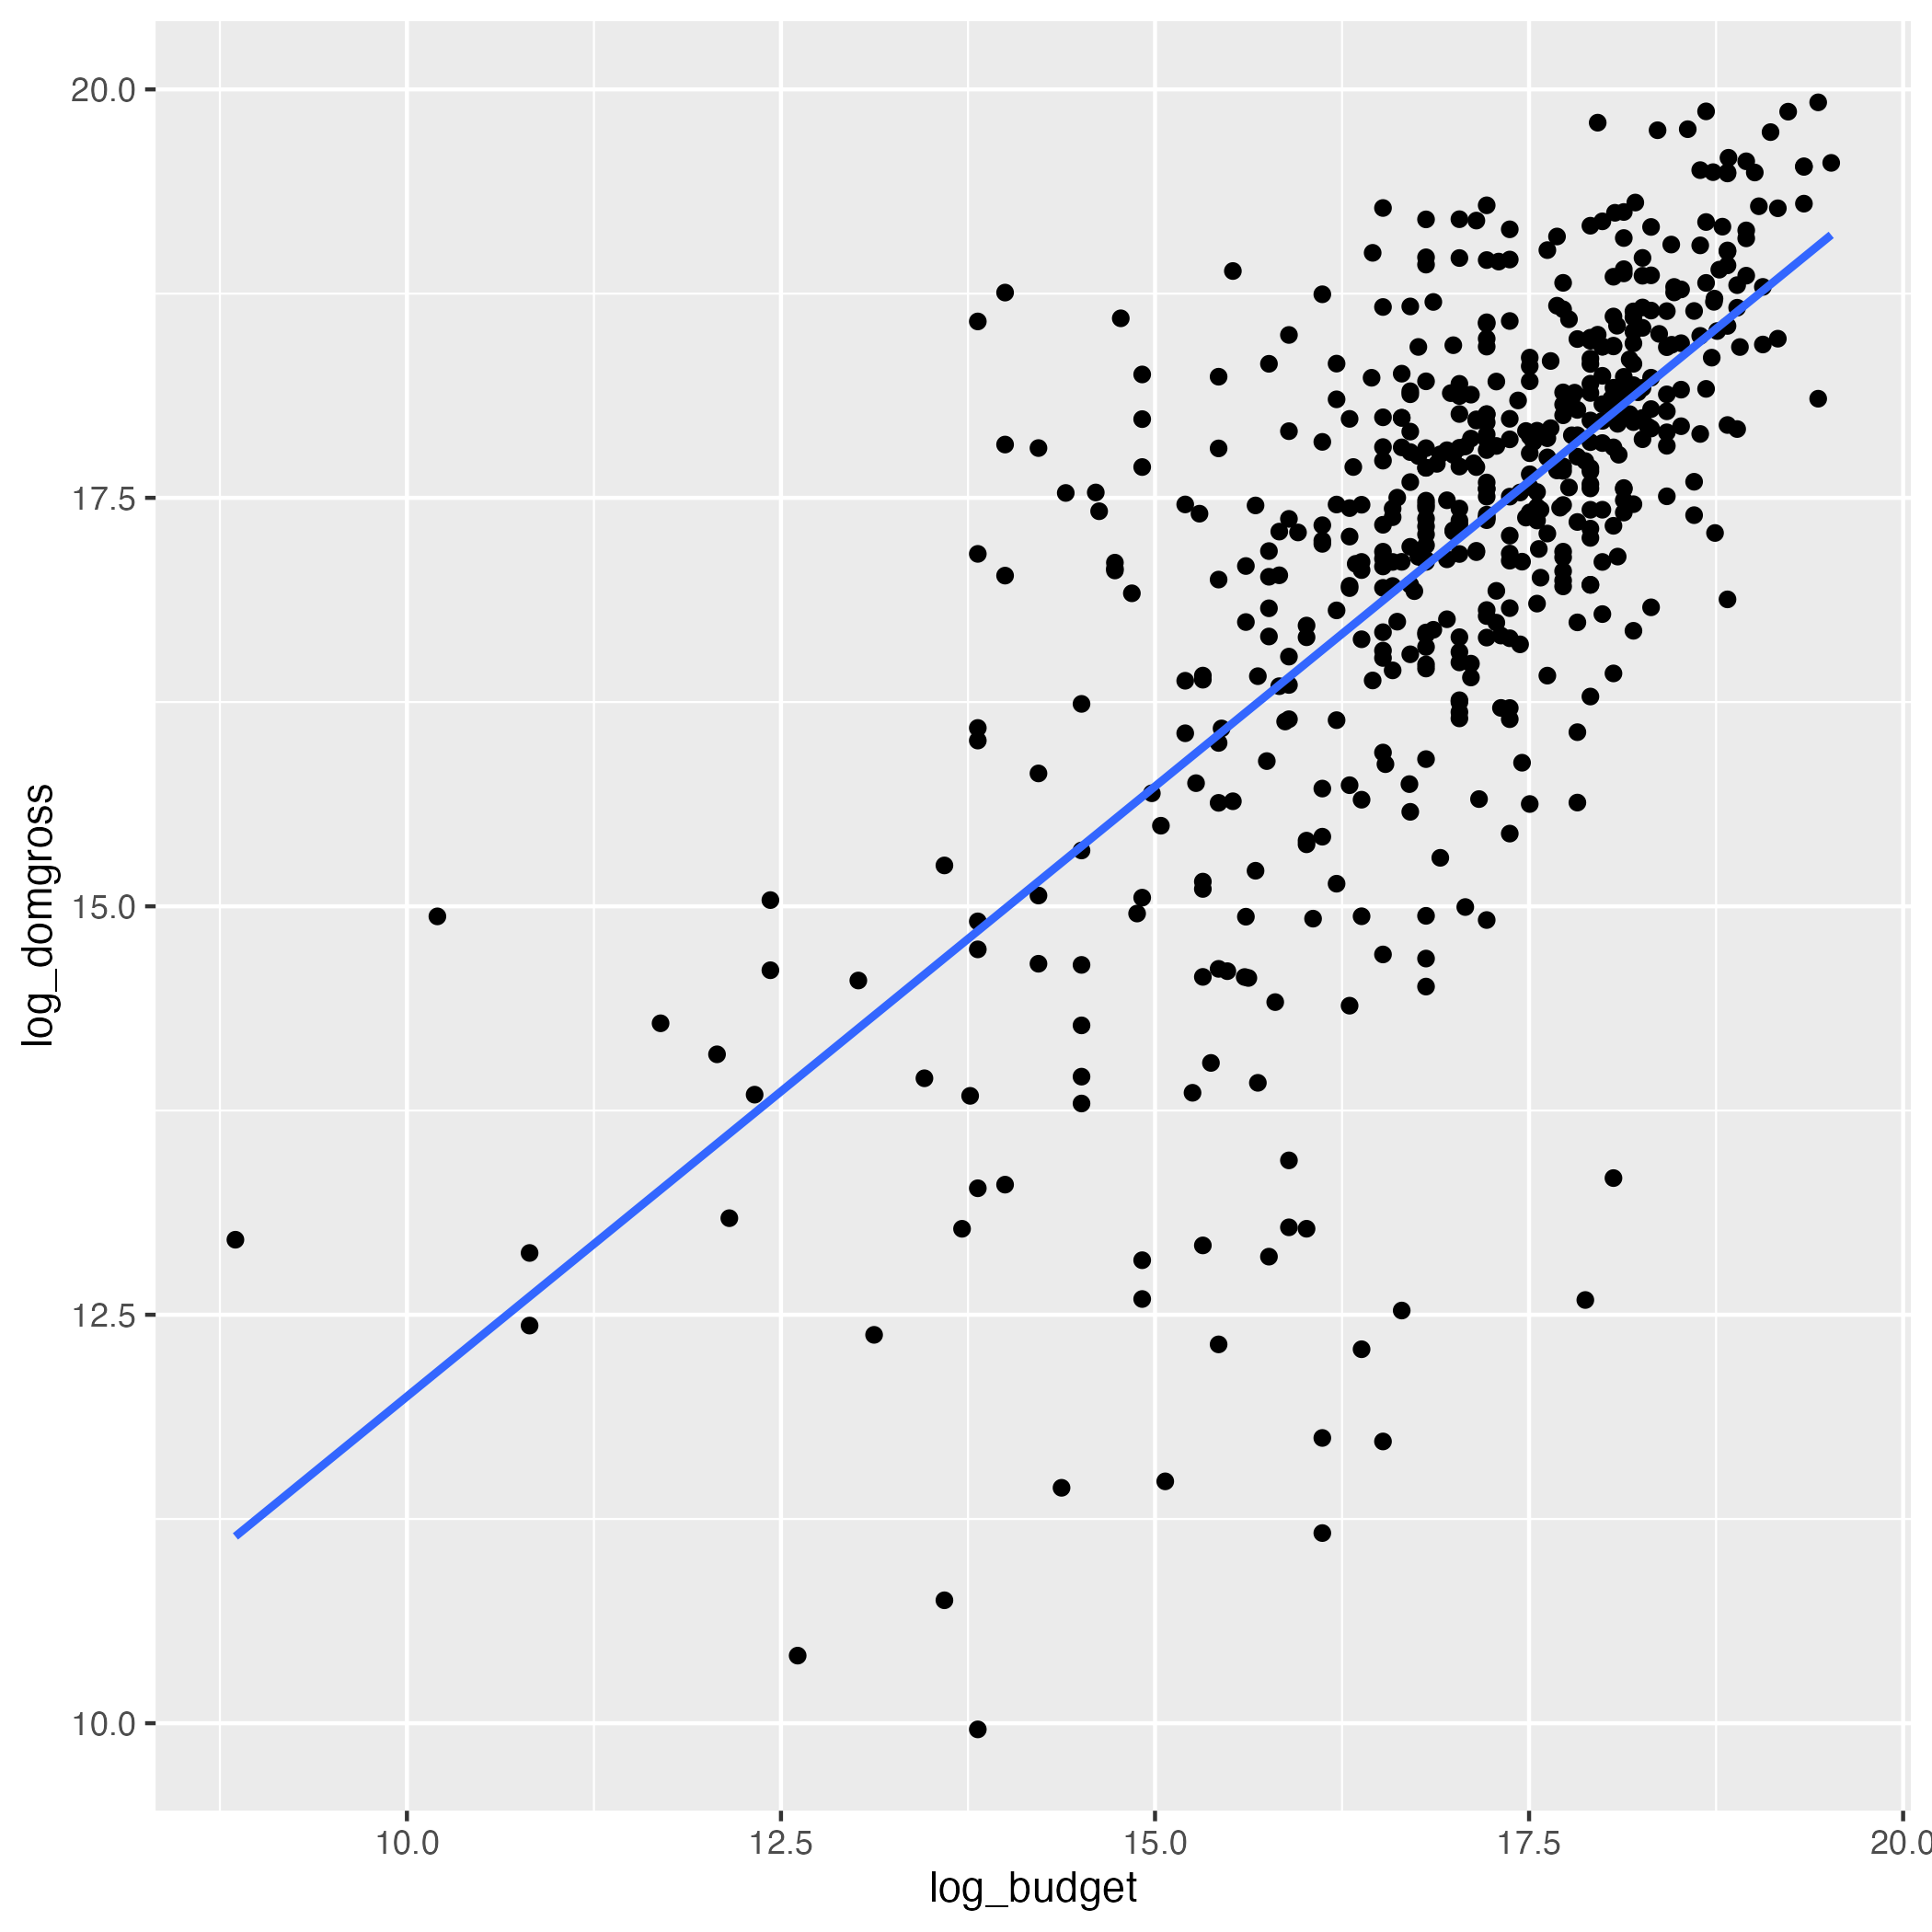
\includegraphics[width=0.65\linewidth,height=4.16667in]{../results/figure5_linear_regression_pred.png}

}

\caption{\label{fig-lm-scatter-pred}Scatterplot of log(movie budget) vs
log(domestic revenue) for the test set}

\end{figure}%

\begin{longtable}[]{@{}llr@{}}

\caption{\label{tbl-lm-metrics}RMSE of the linear regression model}

\tabularnewline

\toprule\noalign{}
.metric & .estimator & .estimate \\
\midrule\noalign{}
\endhead
\bottomrule\noalign{}
\endlastfoot
rmse & standard & 1.266987 \\

\end{longtable}

The RMSE is 1.267. This means on average, the model's predicted log
revenue differs from the actual log revenue by about 1.267. On average,
the predicted revenue can be roughly 3.6 times higher or lower than the
actual revenue.

\subsection{K-Nearest Neighbours Regression
model}\label{k-nearest-neighbours-regression-model}

Below, we also try fitting a K-nearest neighbours (KNN) regression model
using cross-validation to compare whether RMSE might be improved
compared to the linear model. First, we create the recipe and set
log-transformed revenue as our dependent variable and log-transformed
budget as our independent predictor variable, while scaling and
centering the predictor.

Then, we set our model parameters to use KNN for regression, split the
data into 5 folds for cross validation, and create a workflow with our
model and recipe.

\begin{longtable}[]{@{}
  >{\raggedleft\arraybackslash}p{(\linewidth - 12\tabcolsep) * \real{0.1471}}
  >{\raggedright\arraybackslash}p{(\linewidth - 12\tabcolsep) * \real{0.1176}}
  >{\raggedright\arraybackslash}p{(\linewidth - 12\tabcolsep) * \real{0.1618}}
  >{\raggedleft\arraybackslash}p{(\linewidth - 12\tabcolsep) * \real{0.1324}}
  >{\raggedleft\arraybackslash}p{(\linewidth - 12\tabcolsep) * \real{0.0441}}
  >{\raggedleft\arraybackslash}p{(\linewidth - 12\tabcolsep) * \real{0.1471}}
  >{\raggedright\arraybackslash}p{(\linewidth - 12\tabcolsep) * \real{0.2500}}@{}}

\caption{\label{tbl-knn-cv-rmse}Cross-validated RMSE for different K
values in KNN regression (first 6 rows).}

\tabularnewline

\toprule\noalign{}
\begin{minipage}[b]{\linewidth}\raggedleft
neighbors
\end{minipage} & \begin{minipage}[b]{\linewidth}\raggedright
.metric
\end{minipage} & \begin{minipage}[b]{\linewidth}\raggedright
.estimator
\end{minipage} & \begin{minipage}[b]{\linewidth}\raggedleft
mean
\end{minipage} & \begin{minipage}[b]{\linewidth}\raggedleft
n
\end{minipage} & \begin{minipage}[b]{\linewidth}\raggedleft
std\_err
\end{minipage} & \begin{minipage}[b]{\linewidth}\raggedright
.config
\end{minipage} \\
\midrule\noalign{}
\endhead
\bottomrule\noalign{}
\endlastfoot
1 & rmse & standard & 1.817317 & 10 & 0.0580394 & pre0\_mod01\_post0 \\
4 & rmse & standard & 1.503617 & 10 & 0.0372931 & pre0\_mod02\_post0 \\
7 & rmse & standard & 1.428656 & 10 & 0.0401403 & pre0\_mod03\_post0 \\
10 & rmse & standard & 1.401482 & 10 & 0.0367760 & pre0\_mod04\_post0 \\
13 & rmse & standard & 1.394198 & 10 & 0.0385237 & pre0\_mod05\_post0 \\
16 & rmse & standard & 1.394005 & 10 & 0.0425630 & pre0\_mod06\_post0 \\

\end{longtable}

In Table~\ref{tbl-knn-cv-rmse}, we test every 3rd number of neighbours
between 1 and 200, set using tibble(), then filtered for the metric root
mean standard error (RMSE) to evaluate the fit.

\begin{longtable}[]{@{}
  >{\raggedleft\arraybackslash}p{(\linewidth - 12\tabcolsep) * \real{0.1493}}
  >{\raggedright\arraybackslash}p{(\linewidth - 12\tabcolsep) * \real{0.1194}}
  >{\raggedright\arraybackslash}p{(\linewidth - 12\tabcolsep) * \real{0.1642}}
  >{\raggedleft\arraybackslash}p{(\linewidth - 12\tabcolsep) * \real{0.1194}}
  >{\raggedleft\arraybackslash}p{(\linewidth - 12\tabcolsep) * \real{0.0448}}
  >{\raggedleft\arraybackslash}p{(\linewidth - 12\tabcolsep) * \real{0.1493}}
  >{\raggedright\arraybackslash}p{(\linewidth - 12\tabcolsep) * \real{0.2537}}@{}}

\caption{\label{tbl-knn-min}The minimum RMSE.}

\tabularnewline

\toprule\noalign{}
\begin{minipage}[b]{\linewidth}\raggedleft
neighbors
\end{minipage} & \begin{minipage}[b]{\linewidth}\raggedright
.metric
\end{minipage} & \begin{minipage}[b]{\linewidth}\raggedright
.estimator
\end{minipage} & \begin{minipage}[b]{\linewidth}\raggedleft
mean
\end{minipage} & \begin{minipage}[b]{\linewidth}\raggedleft
n
\end{minipage} & \begin{minipage}[b]{\linewidth}\raggedleft
std\_err
\end{minipage} & \begin{minipage}[b]{\linewidth}\raggedright
.config
\end{minipage} \\
\midrule\noalign{}
\endhead
\bottomrule\noalign{}
\endlastfoot
82 & rmse & standard & 1.37301 & 10 & 0.0458433 & pre0\_mod28\_post0 \\

\end{longtable}

In Table~\ref{tbl-knn-min}, we filter the results to get the K value
with the lowest associated RMSE.

\begin{longtable}[]{@{}llrrrl@{}}

\caption{\label{tbl-knn-cv-metrics}Cross-validated RMSE for KNN
regression model at previously found K-value.}

\tabularnewline

\toprule\noalign{}
.metric & .estimator & mean & n & std\_err & .config \\
\midrule\noalign{}
\endhead
\bottomrule\noalign{}
\endlastfoot
rmse & standard & 1.37301 & 10 & 0.0458433 & pre0\_mod0\_post0 \\

\end{longtable}

In Table~\ref{tbl-knn-cv-metrics}, we find the cross-validated RMSE for
the model at K = 82. For the training set, the average RMSE across the
10 folds is 1.37 log units with a standard error of 0.05.

\begin{longtable}[]{@{}llr@{}}

\caption{\label{tbl-knn-summary}RMSE of the KNN regression model}

\tabularnewline

\toprule\noalign{}
.metric & .estimator & .estimate \\
\midrule\noalign{}
\endhead
\bottomrule\noalign{}
\endlastfoot
rmse & standard & 1.287971 \\

\end{longtable}

From Table~\ref{tbl-knn-summary}, the test RMSPE of 1.29 means that, on
average, the KNN model's predicted log revenue differs from the actual
log revenue by about 1.29. On average, the predicted revenue can be
roughly 3.63 times higher or lower than the actual revenue.

So, both KNN and linear regression have similar predictive accuracy,
with linear regression being slightly better.

\begin{figure}

\centering{

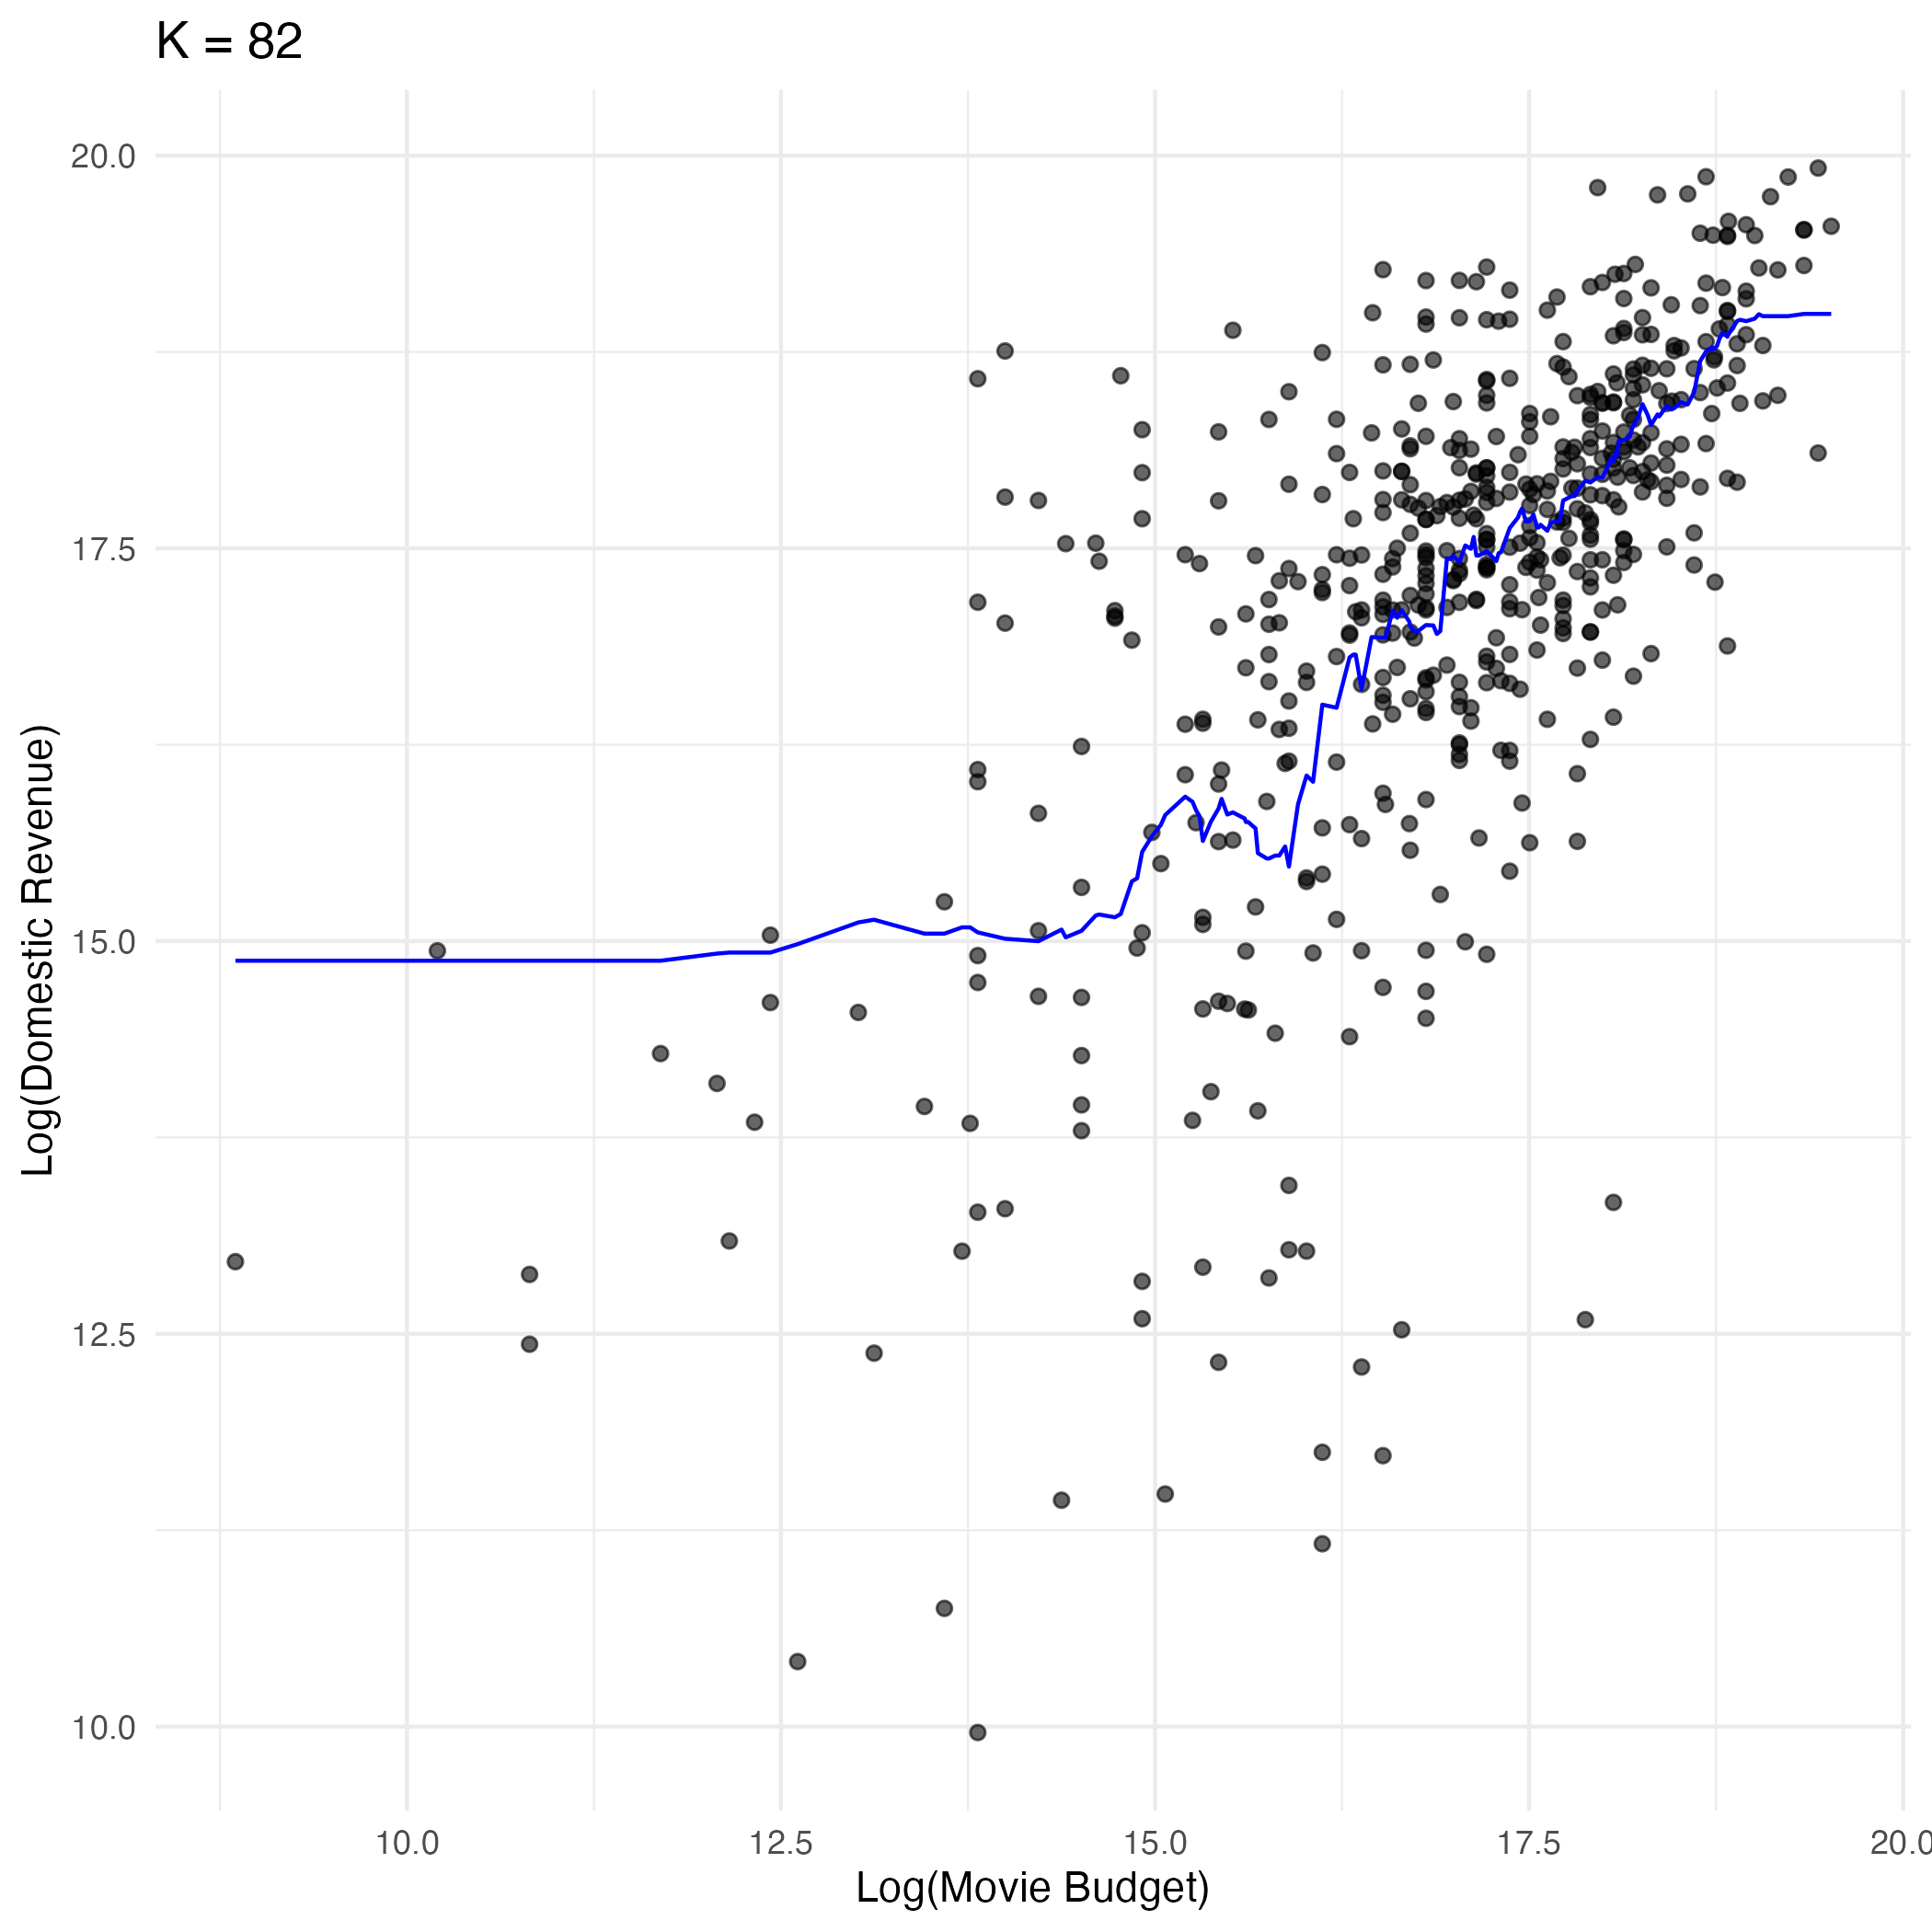
\includegraphics[width=0.65\linewidth,height=4.16667in]{../results/figure6_knn_pred.png}

}

\caption{\label{fig-lm-scatter-pred}Predicted values of log(movie
revenue) (blue line) for the final K-NN regression model}

\end{figure}%

\section{Discussion}\label{discussion}

Our analysis suggests that movie budget is moderately associated with
domestic box office revenue. The exploratory analysis showed a positive
relationship between the two variables, supported by a correlation
coefficient of approximately 0.63, indicating a moderate positive
association. As the raw data is heavily right-skewed, applying a
logarithmic transformation to both variables helped reduce the skewness
and produced a more linear relationship suitable for modelling.

The linear regression model fitted on the log-transformed variables
indicated that log-budget is a statistically significant predictor of
log-revenue. This suggests that increases in movie budget tend to
correspond with increases in domestic box office revenue on average.
When evaluated on the test set, the model produced an RMSPE of
approximately 1.27 log units, meaning predicted revenue may differ from
the true revenue by roughly a factor of 3.55 on average.

To evaluate whether a more flexible model could improve prediction
accuracy, we also trained a KNN model with cross-validation to tune the
number of neighbours. The optimal value with K = 82, producing a test
RMSPE of approximately 1.37, very similar to the linear regression
model. Since KNN did not significantly improve predictive performance,
this suggests that the relationship between log-budget and log-revenue
is reasonably captured by the simpler linear model. Consistent with
previous research on film economics, our results suggest that while
budget is associated with higher revenue, it alone cannot fully explain
the variability in box office outcomes (Prag and Casavant 1994).

Despite the observed relationship, a couple of limitations exist in this
analysis. First, the models only consider budget as a single predictor,
when movie revenue is likely influenced by many additional factors such
as marketing, release timing, critical reception, and star power.
Second, the dataset only includes domestic revenue, where particular
films may have performed differently internationally.

Future work could improve predictive performance by incorporating
additional variables such as genre, production studio, critical
reception, and by analyzing worldwide revenue rather than only domestic.
More advanced modeling techniques such as random forests or gradient
boosting models may also capture nonlinear relationships between
features and revenue.

Overall, our findings suggest that movie budget does have a moderate
predictive relationship with domestic revenue, but it is not a complete
predictor of financial success.

\section*{Citations}\label{citations}
\addcontentsline{toc}{section}{Citations}

\phantomsection\label{refs}
\begin{CSLReferences}{1}{0}
\bibitem[\citeproctext]{ref-basuroy2003critical}
Basuroy, Suman, Subimal Chatterjee, and S. Abraham Ravid. 2003. {``How
Critical Are Critical Reviews? The Box Office Effects of Film Critics,
Star Power, and Budgets.''} \emph{Journal of Marketing} 67 (4): 103--17.
\url{https://doi.org/10.1509/jmkg.67.4.103.18692}.

\bibitem[\citeproctext]{ref-devany1999uncertainty}
De Vany, Arthur, and W. David Walls. 1999. {``Uncertainty in the Movie
Industry: Does Star Power Reduce the Terror of the Box Office?''}
\emph{Journal of Cultural Economics} 23 (4): 285--318.

\bibitem[\citeproctext]{ref-fivethirtyeight2014bechdel}
FiveThirtyEight. 2014. {``Bechdel Test Movie List.''}
\url{https://github.com/fivethirtyeight/data/tree/master/bechdel}.

\bibitem[\citeproctext]{ref-prag1994empirical}
Prag, Jay, and James Casavant. 1994. {``An Empirical Study of the
Determinants of Revenues and Marketing Expenditures in the Motion
Picture Industry.''} \emph{Journal of Cultural Economics} 18 (3):
217--35.

\end{CSLReferences}




\end{document}
